\chapter{PERATURAN UMUM}
\section{Pendahuluan}
Pendidikan profesional bertujuan untuk menghasilkan tenaga kerja yang siap pakai. Lulusan yang siap pakai adalah ciri yang membedakan antara pendidikan profesional dengan pendidikan akademis. Selama masa pendidikan, mahasiswa Politeknik Pos Indonesia dipersiapkan dan dilatih agar kelak mempunyai kemampuan untuk beradaptasi secepatnya dengan dunia kerja.

Untuk melatih mahasiswa Politeknik Pos Indonesia dalam hal implementasi serta mewujudkan hasil implementasinya, mahasiswa diwajibkan mengerjakan Proyek Program Analisis Aplikasi. Dengan tugas tersebut diharapkan mahasiswa dapat menerapkan ilmu dan pengetahuan yang telah dipelajari sebelumnya. Diharapkan pula, mahasiswa mampu mengidentifikasi persoalan, implementasi, menentukan spesifikasi,serta mampu mengukur dan mencari kesalahan (\textit{trouble shooting}) hasil yang di implementasikannya.

\section{Nama Kegiatan}
\textbf{PROYEK PEMROGRAMAN DAN JARINGAN }

\section{Tujuan}
Proyek Program Aplikasi, Pemrograman dan Jaringan termasuk mata kuliah yang harus ditempuh sebagaimana mata-mata kuliah lainnya pada program pendidikan Diploma IV Politeknik Pos Indonesia yang bertujuan memberikan kesempatan kepada mahasiswa untuk mengimplementasikan pengetahuan teori dan praktek yang didapat dalam bentuk suatu pekerjaan proyek.\textit{ Dengan menambahkan fitur web service dan network security}.\textbf{Web service wajib menggunakan Oauth atau sistem Token buatan sendiri}. Database menggunakan fungsi dan atau prosedur dan atau trigger. Penggunaan atau implementasi database cache pada aplikasi proyek 2 menggunakan \textbf{redis} akan menjadi nilai lebih.

\section{Waktu}
Proyek Pemrogram dan Jaringan  dikerjakan pada semester 3.

\section{Tahap-Tahap Pelaksanaan Proyek}
Dalam melakukan pelaksanaan	proyek harus berdasarkan tahapan-tahapan	yang dijelaskan	sebagai	berikut	:
\begin{enumerate}
\item Pemilihan topik dari proyek yang akan dikerjakan ;

\item Pengajuan proposal proyek ke dosen calon pembimbing yang telah ditentukan sebelumnya oleh koordinator proyek ;

\item Proses review oleh dosen calon pembimbing	untuk disetujui, kemudian proposal dikumpulkan ke	prodi untuk	mendapatkan	form nilai	bimbingan proyek II ;

\item Proses bimbingan yang	berkaitan dengan pembuatan aplikasi	dan penyusunan laporan yang diarahkan oleh dosen pembimbing masing-masing	untuk diberikan pengesahan penilaian proses	bimbingan perminggu.

\item Pelaksanaan sidang untuk menguji dan menilai hasil akhir dari	 kegiatan proyek yang dilakukan sebelumnya.
\end{enumerate}

\section{Proses Pemilihan Topik Proyek}
Topik Proyek dapat berasal dari	mahasiswa atau pembimbing proyek II.	 Prosedur pemilihan topik untuk keduanya	adalah sebagai berikut :


\begin{figure}[H]
    \centering
    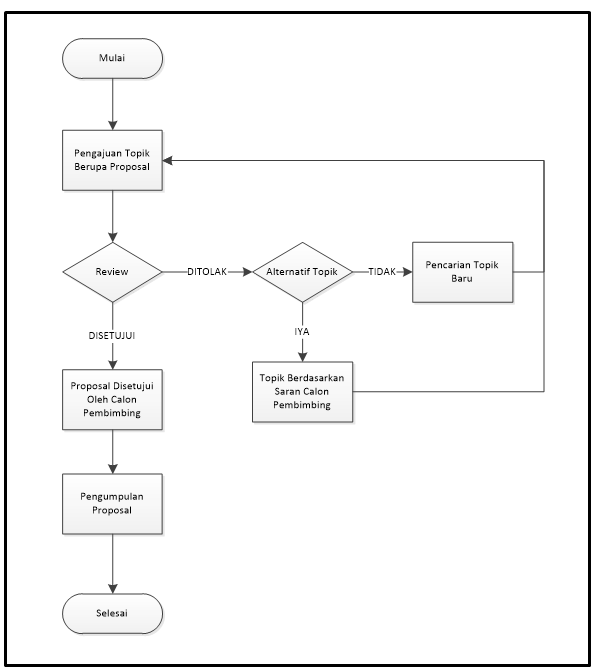
\includegraphics[scale=0.7]{figures/alur.png}
    \caption{Diagram Alir Pemilihan dan Pengajuan Topik}
    \label{alir}
\end{figure}

\section{Pengajuan Topik dan Penetapan Pembimbing Proyek}
Topik diajukan ke Koordinator Proyek dengan	menggunakan	proposal dalam	bentuk \textbf{luring dan daring}. Berdasarkan hasil penilaian \textit{reviewer}, maka Koordinator Proyek menerima atau menolak proposal yang diajukan dan menetapkan pembimbing (Lihat \textit{Flowchart} Proses Pengajuan hingga Sidang Proyek).

\section{Peraturan Pelaksanaan Proyek II}
Dalam pelaksanaan Proyek II	ini	ada	beberapa aturan	yang ditentukan	diantaranya	sebagai	berikut	:

\begin{enumerate}
	\item Telah	 Mengikuti	 dan	 lulus	 pada	 Kegiatan	 Character	 Building	 di	 Politeknik	 Pos Indonesia yang	dikuatkan	dengan	melampirkan	Fotocopy	Sertifikat.
	
	\item Telah	Mengikuti	 dan	lulus	 pada	 Kegiatan	MORRIS	 Program	 Studi	 Teknik	 Informatika yang dikuatkan	dengan	melampirkan	Fotocopy	Sertifikat.
	
	\item Lulus	minimal	C	untuk	4	mata	kuliah	Web	Service,	Basdat,	RPL, Jarkom, Mobile, Metlid, Admin	Jarkom.
	
	\item Pada	 saat	 pengumpulan	 proposal	 disertakan	 KRS	 dan	 DHS, yang langsung dikumpulkan	di	admin.
	
	\item Satu kelompok terdiri atas maksimal 2 orang dan memiliki 1 tema.
	
	\item Jika terlambat mengumpulkan Proposal (tidak sesuai dengan	jadwal yang telah	ditentukan) maka	 akan	 dinyatakan	\textbf{TIDAK LULUS} dan	 tidak	 diperkenankan	 mengajukan	 judul kembali.	\textit{\textbf{(dianggap mengulang proyek pada semester berikutnya)}} ;
	
	\item Jika Proposal	yang ditolak maka diberikan waktu 1 minggu untuk pengajuan ulang	Proposal	Proyek	II,	jika penolakan	melebihi 3	kali maka dinyatakan	\textbf{TIDAK LULUS} dan tidak	 diperkenankan	 mengajukan judul kembali. \textit{\textbf{(dianggap mengulang proyek pada semester berikutnya)}} ;
	
	\item Penilaian	Proses	Bimbingan	:	Diberikan	total	waktu selama 10 minggu, setiap minggu	mendapat 1 penilaian proses	bimbingan dengan	nilai sebesar maksimal 10 terdiri dari penilaian \textit{ uniqeness} 300	 kata tulisan blog (50\%), 10 \textit{commit} standard github (25\%), dan video log standard (25\%) yang berisi tentang pengerjaan pada waktu minggu tersebut, keterlambatan pengerjaan tidak akan mendapatkan toleransi ( Nilai 0 ). Sehingga nilai total untuk 10 minggu jumlahnya 100. Jika nilai total bimbingan kurang dari 80 maka dianggan \textbf{TIDAK LULUS} dan tidak diperkenankan mengajukan judul kembali. \textit{\textbf{(dianggap mengulang proyek pada semester berikutnya)}} ;
	
	\item Jika terlambat mengumpulkan \textit{Form} Nilai Bimbingan ( melewati tanggal yang telah ditentukan )  maka dianggan \textbf{TIDAK LULUS} dan tidak diperkenankan mengajukan judul kembali. \textit{\textbf{(dianggap mengulang proyek pada semester berikutnya)}} ;
	
	\item Jika Pengumpulan Draf Laporan untuk proses sidang dan kelengkapan	lainnya tidak dikumpulkan di staff Prodi D4-Teknik Informatika	atau terlambat maka	sidang akan	dijadwalkan	belakangan	dan \textit{\textbf{Bobot	nilai	akan dikurangi	20	Point}}	.	
	
	\item Perubahan	 jadwal	 sidang	 dikarenakan	 hal-hal	 yang	 dapat	 dipertanggung	 jawabkan maka	 peserta	 sidang	 melakukan	 proses	 pengajuan	 perubahan	 jadwal	 sidang	 dengan	persetujuan	 dosen	pembimbing,	penguji	 dan	 koordinator	 disertai	 form pengajuan	
perubahan	sidang. jika tidak dapat dipertanggung	jawabkan	dinyatakan \textbf{TIDAK	LULUS}  dan tidak diperkenankan mengajukan judul kembali. \textit{\textbf{(dianggap mengulang proyek pada semester berikutnya)}} ;
	
\end{enumerate}

\par Mengenai keterlambatan	 dalam	 pengajuan	 topik	 akan berakibat menghambat kegiatan proyek yang	akan dilakukan.	Dikarenakan	kegiatan	memiliki jadwal	yang telah ditentukan,maka diharapkan tiap-tiap mahasiswa memperhatikan jadwal pengajuan topik agar tidak menghambat jadwal kegiatan	lainnya. Pengerjaan	proyek	membutuhkan	proses dan	waktu yang	cukup	lama sehingga harap	diperhatikan baik-baik.

\section{Jadwal Pelaksanaan Proyek II}
Jadwal	 pelaksanaan proyek	 II	 dilaksanakan	 pada	 semester	 perkuliahan yang telah	ditentukan.	 Lama	 kegiatan	 proyek	 adalah	 1 semester. Berikut tabel	 kegiatan yang	dilakukan	pada	kegiatan	proyek	untuk	semester	ganjil	tahun	ajaran	2019-2020 :


% Please add the following required packages to your document preamble:
% \usepackage[normalem]{ulem}
% \useunder{\uline}{\ul}{}
\begin{table}[]
\caption*{JADWAL KEGIATAN PROYEK II\\
PROGRAM STUDI D4 TEKNIK INFORMATIKA TAHUN AJARAN 2019/2020}
\label{jadwal}
\begin{adjustbox}{width=\textwidth}
\begin{tabular}{|l|l|l|l|}
\hline
\multicolumn{1}{|c|}{No} & \multicolumn{1}{c|}{Hari/Tanggal} & \multicolumn{1}{c|}{Kegiatan} & \multicolumn{1}{c|}{Keterangan} \\ \hline
1 & 7 Oktober 2019 & Sosialisasi Kegiatan Proyek II & -        Sosialisasi Kegiatan Proyek II dilaksanakan pada pukul 13.00 di ruang 113. \\ \hline
2 & 17-19 Oktober 2019 & \begin{tabular}[c]{@{}l@{}}Pengajuan Proposal + \\ Review Proposal\end{tabular} & \begin{tabular}[c]{@{}l@{}}-        Proposal diajukan ke Prodi dalam bentuk daring dan luring untuk direview dan disetujui.\\ \\ -        Jika Proposal DITOLAK maka diberikan waktu 3 hari untuk ulang Proposal Proyek II \\ dikumpulkan di Staff Admin Prodi DIV Teknik Informatika, jika penolakan Melebihi 3 kali, \\ maka dianggap TIDAK LULUS dan tidak diperkenankan mengajukan judul kembali. \\ (dianggap mengulang Proyek di semester berikutnya) \\ \\ -        Pengumpulan Proposal dapat dilakukan setiap hari kerja mulai jam 09.00-15.00\end{tabular} \\ \hline
3 & \begin{tabular}[c]{@{}l@{}}24 Oktober 2019 s.d\\ 13 Januari 2020\end{tabular} & \begin{tabular}[c]{@{}l@{}}Proses Bimbingan \\ menggunakan sistem\\ kendali mingguan\\ Selama 10 minggu.\\ Setiap minggu\\ terdapat penilaian\end{tabular} & \begin{tabular}[c]{@{}l@{}}-        Mahasiswa melakukan proses bimbingan kepada dosen pembimbing masing-masing dengan membawa\\ Form Nilai Bimbingan dan Buku Pedoman Proyek (WAJIB DICETAK)\\ \\ -        Mahasiswa yang memiliki dosen pembimbing yang sama, membentuk grup whatsapp \\ dengan mengangkat satu orang admin, dan grup diberi nama " Proyek 2 ",admin akan \\ melakukan undangan ke grup tersebut kepada mahasiswa yang memiliki pembimbing\\ yang sama dan pembimbing itu sendiri.\\ \\ -        Sebelum melakukan pertemuan bimbingan, peserta wajib memposting di grup whatsapp \\ yaitu link blog (50\%) laporan yang didalamnya sudah termasuk video standar (25\%) dan\\ 10 commit git (25\%) pada minggu tersebut untuk dinilai, penilaian akan dibantu oleh \\ admin grup whatsapp,\\ \\ -        Proses bimbingan menggunakan sistem kendali mingguan yang sudah disediakan.\end{tabular} \\ \hline
4 & 16-18 Januari 2020 & \begin{tabular}[c]{@{}l@{}}Pengumpulan Draft\\ Laporan Proyek II\end{tabular} & \begin{tabular}[c]{@{}l@{}}-        Pengumpulan Draft Laporan Proyek II telah di setujui oleh pembimbing dengan  \\ mengumpulkan  dokumen sebagai berikut :\\ \\ -        Draft Laporan Proyek II (dua rangkap)\\ \\ -        Lembar pernyataan dan permohonan sidang Proyek II yang telah disetujui \\ oleh pembimbing (dua rangkap)\\ \\ -        Lembar Persetujuan Sidang (2 rangkap)\\ \\ -        Form nilai bimbingan dengan syarat nilai minimal 80.\\ \\ -        Pengumpulan dilakukan di Staff Admin Prodi DIV­‐Teknik Informatika setiap hari kerja \\ mulai  jam  09.00 ‐ 15.00, untuk keterlambatan akan dikenakan sanksi sesuai dengan ketentuan\\ dan kebijakanyang telah diatur.\\ \\ -        Kelengkapan repositori githubstandar meliputi, dokumen, kode, manual screenshot performansi commit \\ dilampirkan di lampiran laporan.\end{tabular} \\ \hline
5 & \begin{tabular}[c]{@{}l@{}}30 Januari s.d\\ 10 Februari 2020\end{tabular} & Sidang Proyek I & \begin{tabular}[c]{@{}l@{}}-       Apabila pada saatsidang mahasiswa berhalangan hadir dan tidak hadir tepat waktu,\\ maka sidang dibatalkan dan dinyatakan TIDAK LULUS\\ \\ -       Pada saat sidang mahasiswa mempersiapkan peralatan sidang 30 menit sebelum sidang.\\ \\ -       Apabila tidak melaksanakan revisi tepat waktu 1 minggu maka dinyatakan TIDAK LULUS.\end{tabular} \\ \hline
6 & 20-22 Februari 2020 & \begin{tabular}[c]{@{}l@{}}Pengumpulan \\ Distribusi CD dan \\ Jurnal Proyek II\end{tabular} & \begin{tabular}[c]{@{}l@{}}-       Pengumpulan dilakukan di ruang Staff Admin  Prodi  DIV-­Teknik  Informatika setiap  hari  kerja  \\ mulai  jam  09.00‐15.00, untuk keterlambatan akan dikenakan sanksi sesuai dengan ketentuan\\ dan kebijakan yang telah diatur.\\ \\ -       Kelengkapan Blog, github dan video sudah 100\%.\\ \\ -       Apabila terlambat mengumpulkan pendistribusian Laporan Proyek, CD dan Jurnal Proyek, \\         maka NILAI DIKURANGI satu tingkat (Contoh: dari B ke C)\end{tabular} \\ \hline
\end{tabular}
\end{adjustbox}
\end{table}